\documentclass{beamer}
  \usepackage{graphicx}
  \usepackage{amsmath,amsthm, amssymb}
  \usepackage{multicol}
  \usepackage{lipsum}
  \boldmath
  \usetheme{gemini}
  \usecolortheme{grazmini}
  \usepackage[orientation=portrait,size=a0,scale=1.4]{beamerposter}

\newcommand{\compresslist}{
        \setlength{\itemsep}{0pt}%
        \setlength{\parskip}{1pt}%
        \setlength{\parsep}{0pt}%
}

% If you have N columns, choose \sepwidth and \colwidth such that
% (N+1)*\sepwidth + N*\colwidth = \paperwidth
\newlength{\sepwidth}
\newlength{\colwidth}
\setlength{\sepwidth}{0.025\paperwidth}
\setlength{\colwidth}{0.3\paperwidth}

\newcommand{\separatorcolumn}{\begin{column}{\sepwidth}\end{column}}

\graphicspath{{pics/}}

  % == Title ====================

	\logoleft{\begin{minipage}{.9\linewidth}
        
\includegraphics[width=\linewidth]{didip_sm.png}
		\vspace{.2em}\\
        
\includegraphics[width=\linewidth]{logo_erc-flag_eu.png}
\end{minipage}}

  \title[Beamer Poster]{This Is A Rather Long Title For A Digital Humanities Poster Presentation}

  \author[first.author@uni-graz.at]{First Author \inst{1} \and Second Author \inst{2}}
 
  \institute[University of Graz]
  {\inst{1} Department of Digital Humanities, University of Graz \samelineand \inst{2} History Department, University of Graz}
  \date{\today}
  
  \logoright{
\includegraphics[width=\linewidth]{unigraz_logo}}
% For more than one logo (eg. partnership with TU), eg.
%	\logoright{\begin{minipage}{\linewidth}
%        
\includegraphics[width=\linewidth]{unigraz_logo}
%		\vspace{.2em}\\
%        \includegraphics[width=\linewidth]{TU_logo}
%        \end{minipage}}


  %%%%%%%%%%%%%%%%%%%%%%%%%%%%%%%%%%%%%%%%%%%%%%%%%%%%%%%%%%%%%%%%%%%%%%%%%%%%%%%%%5
\begin{document}
\begin{frame}{} 
    	\vfill
	\begin{block}{\large Introduction}
		\lipsum*[19]
		\vspace{1em}

		%\setlist{nolistsep} % makes space above the list tighter
		\begin{minipage}{.48\linewidth}
			\textbf{Challenges:}
			\begin{itemize}
		    \compresslist % more compact list items
				\item Ex sapien vitae pellentesque sem placerat in id.
				\item Pretium tellus duis convallis tempus leo eu aenean.
			\end{itemize}
		\end{minipage}%
		\hfill\vline\hfill%
		\begin{minipage}{.48\linewidth}
			\textbf{Constraints:}
			\begin{itemize}
		    \compresslist
				\item Montes nascetur ridiculus mus donec rhoncus eros lobortis.
		    \item Aenean sed diam urna tempor pulvinar vivamus fringilla. 
				\end{itemize}
		\end{minipage}
   	\end{block}
   	\vfill
   	\begin{columns}[t]
		\separatorcolumn
    		\begin{column}{.63\linewidth}
			\begin{columns}[t,totalwidth=\linewidth]
				\begin{column}{.49\linewidth}
					\begin{block}{Figure}
						\small
						This is an actual \LaTeX{} figure:
						% the 'figure' environment _may_ occur in a block
						\begin{figure}
						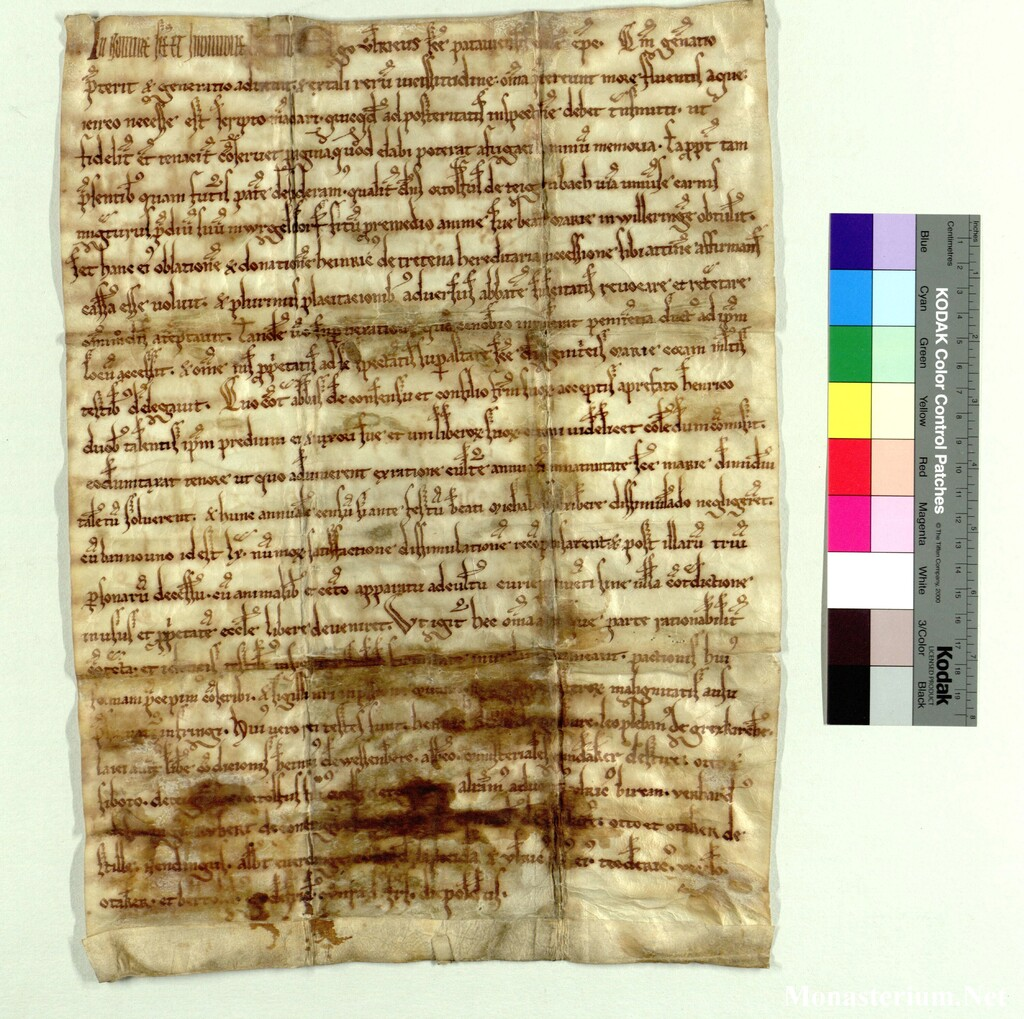
\includegraphics[width=.5\textwidth]{9bde06a84833576b4027ae6331553753.img.jpg}\\
						\caption{A charter}
						\end{figure}

						\lipsum*[2][1-5]
					\end{block}
				\end{column}
				\separatorcolumn
				\begin{column}{.49\linewidth}
					\begin{block}{Text block}
						\lipsum*[5]
						\lipsum*[7][5-8]
					\end{block}
				\end{column}
				%\separatorcolumn
			\end{columns}
			\begin{block}{Two-column text, with compact lists}
				\small
				\begin{multicols}{2}
					A list:
					\begin{itemize}
					\compresslist
						\item Etiam volutpat sem sed felis pulvinar consequat.
						\item In lobortis mi nec nulla dictum, sed interdum sapien scelerisque.
						\item Nam non nulla at lectus rhoncus lacinia.
					\end{itemize}
				    \lipsum[1-2]
				\end{multicols}
			\end{block}
			\begin{block}{PDF Plots}
					\begin{minipage}{.48\linewidth}
					\small
					\lipsum[5]
					\end{minipage}\hfill
					\begin{minipage}{.48\linewidth}
					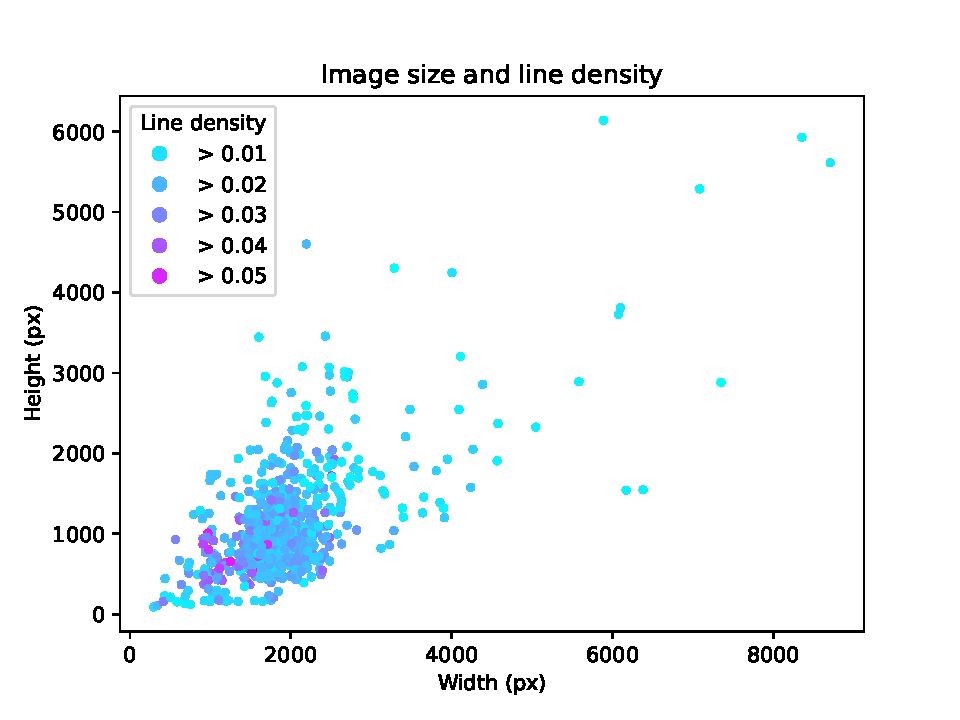
\includegraphics[width=\textwidth]{img_size_scatter_plot.pdf}
					\end{minipage}%
			\end{block}
      		\end{column}
		\separatorcolumn
		\begin{column}{.33\linewidth}
			\begin{block}{Vertical Span}
				\lipsum[10-12]

				\lipsum*[1][9-11]
			\end{block}
			\begin{block}{References}
			\nocite{*}
			\bibliographystyle{plain}
			\bibliography{poster}
				\vspace{.1em}
				\centering
				\begin{tabular}{cc}
				
\includegraphics[width=.3\linewidth]{pics/qr_monasterium.png} &
        				
\includegraphics[width=.3\linewidth]{pics/qr_didip.png} \\
				Monasterium &
       	 				DiDip
				\end{tabular}
			\end{block}
      		\end{column}
		\separatorcolumn
   	\end{columns}
  \end{frame}
\end{document}


